\chapter{linear algebra review} \label{A}
\begin{itemize}
	\item \textbf{def.:} an \textbf{algebra} (over a field $K$) is a vector space $+$ bilinear product $B : A \times A \rightarrow \mathcolor{red}{A}$ (简写做 $\cdot$), 几个主要特征如下,
	\begin{enumerate}
		\item 双线性形式 $B(\cdot, \cdot)$ 满足左, 右分配律和 \eqref{A.0.2},
		
		\item 可能存在单位元 (不是零向量),
		\begin{equation}
			B(e, x) = x, \forall x
		\end{equation}
		存在单位元的代数称为 \textbf{unital algebra}.
	\end{enumerate}
	
	\item 注意区分 bilinear form 和 sesquilinear form,
	\begin{equation} \label{A.0.2}
		\begin{dcases}
			B(a x, b y) = a b B(x, y) & \text{双线性} \\
			S(a x, b y) = a^* b S(x, y) & \text{半双线性, 有复共轭}
		\end{dcases}
	\end{equation}
	一般用 $(\cdot, \cdot)$ 和 $\braket{\cdot, \cdot}$ 区分.
	
	\noindent\rule[0.5ex]{\linewidth}{0.5pt} % horizontal line
	
	\item 李代数 $\mathfrak{g}$ 一定不存在单位元, (因为一定有 $[E, E] = 0 \Longrightarrow E = 0$ 与单位元性质矛盾).
	
	\noindent\rule[0.5ex]{\linewidth}{0.5pt} % horizontal line
	
	\item 另外,
	\begin{equation}
		\begin{array}{rcl}
			\text{injective} & \leftrightarrow & \text{one-to-one function} \\
			\text{surjective} & \leftrightarrow & \text{onto} \\
			\text{bijective} & \leftrightarrow & \text{one-to-one correspondence}
		\end{array}
	\end{equation}
	
	\item a exact sequence (其中 $f_i$ 都是 homomorphism),
	\begin{equation}
		G_1 \overset{f_1}{\rightarrow} G_2 \overset{f_2}{\rightarrow} G_3 \cdots
	\end{equation}
	表示 $f_1[G_1] = \ker(f_2)$. 例如,
	\begin{itemize}
		\item $G \rightarrow H \rightarrow 0$ 表示 $f[G] = \ker(f_2) = H$, 即 $f$ 是 onto.
		
		\item $0 \rightarrow G \rightarrow H$ 表示 $\{0\} = \ker(f)$, 即 $f$ 是 one-to-one.
	\end{itemize}
	
	\item a short exact sequence,
	\begin{equation}
		0 \rightarrow G_1 \overset{f_1}{\rightarrow} G_2 \overset{f_2}{\rightarrow} G_3 \rightarrow 0
	\end{equation}
	表示 $f_1$ 是 one-to-one, $f_2$ 是 onto, 且 $\ker(f_2) = f_1[G_1]$, 所以,
	\begin{figure}[H]
		\centering
		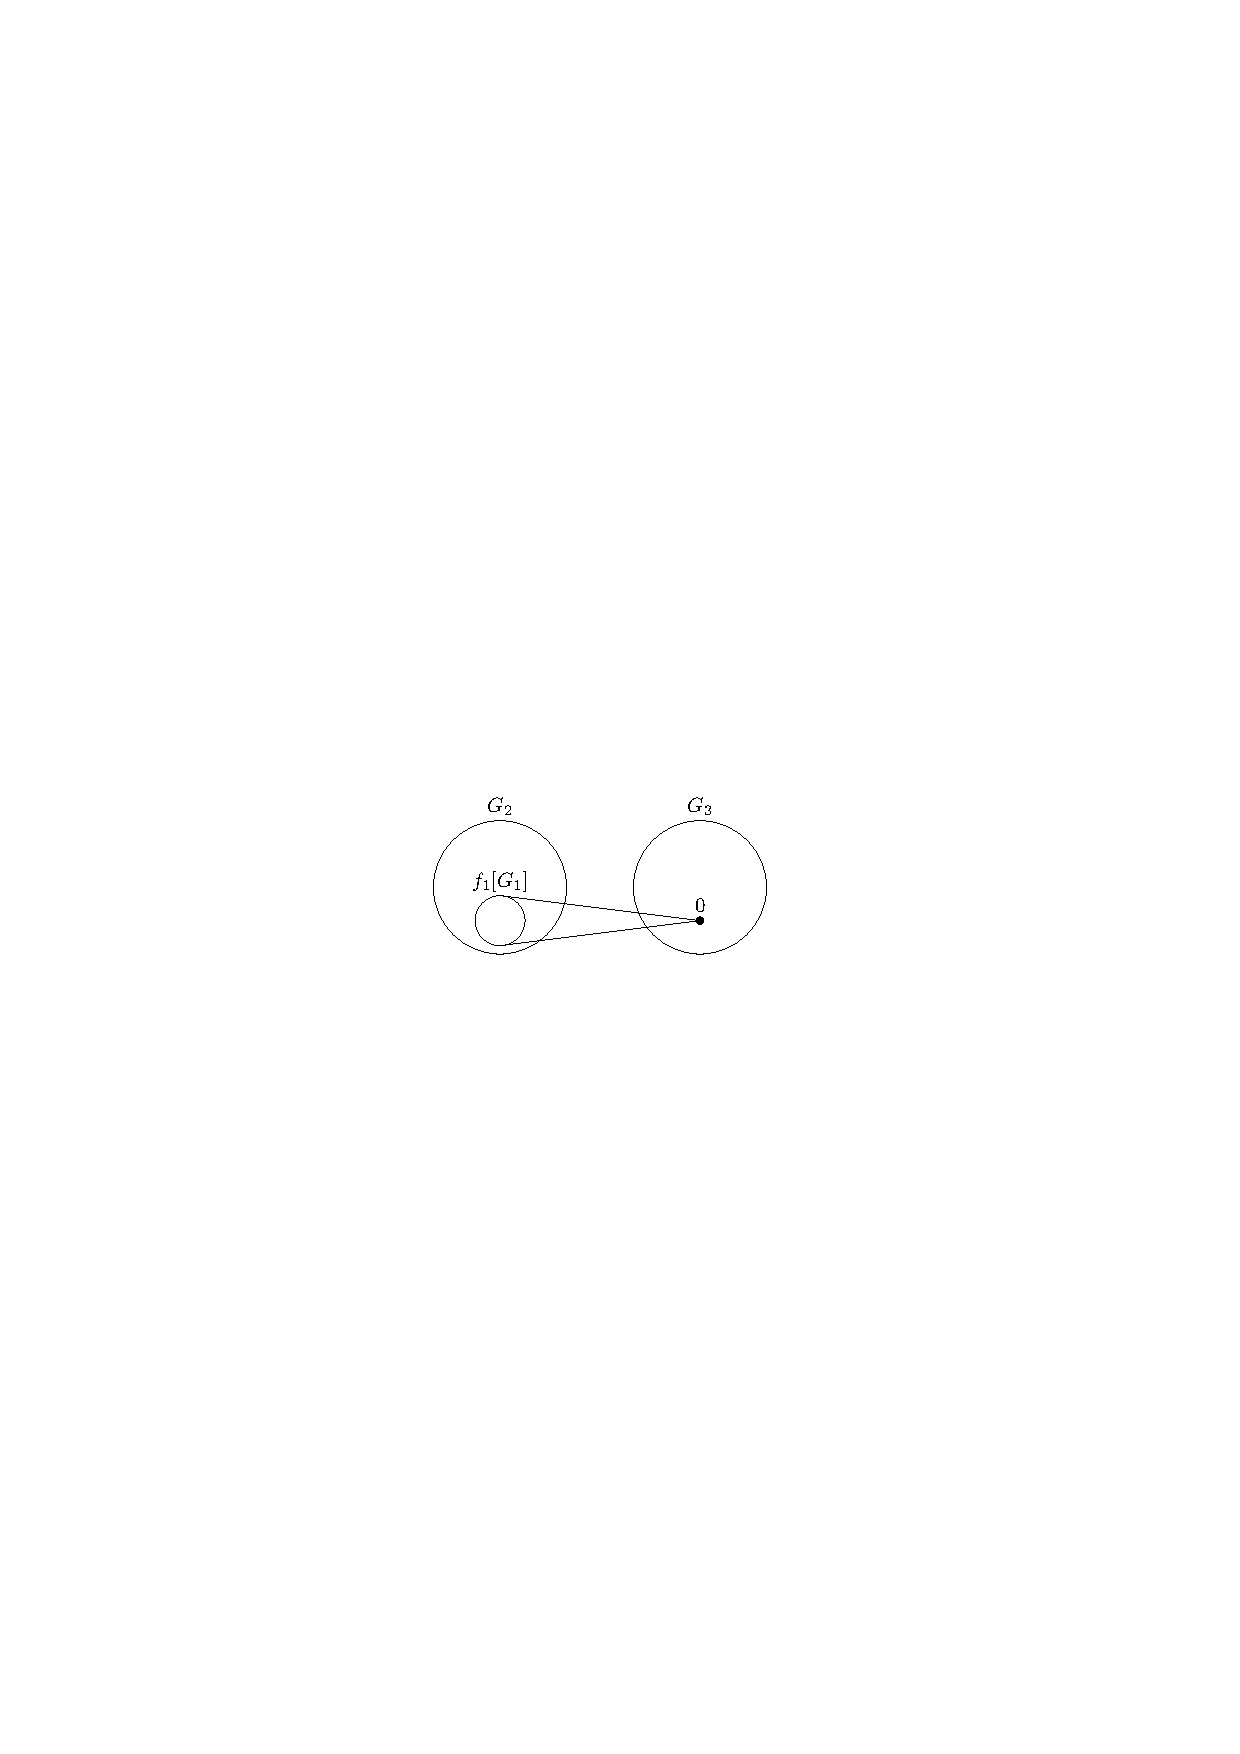
\includegraphics[scale=1]{figures/short exact sequence.pdf}
	\end{figure}
	
	注意到 $f_1, f_2$ 都是 homomorphism, 所以,
	\begin{equation}
		G_3 = G_2 / f_1[G_1]
	\end{equation}
\end{itemize}

\section{eigenvalues and eigenspaces} \label{A.1}
\begin{itemize}
	\item eigenvectors associated to different eigenvalues are linearly independent.
	
	\begin{tcolorbox}[title=proof:]
		if $v_1, \cdots, v_k$ are linearly independent eigenvectors with different eigenvalues, and $v_{k + 1}$ is a linear combination of them and is also an eigenvector, then,
		\begin{align}
			&v_{k + 1} = \sum_{i = 1}^k c^i v_i \Longrightarrow \lambda_{k + 1} v_{k + 1} = \sum_i c^i \lambda_i v_i \notag \\
			\Longrightarrow & 0 = \sum_i c^i (\lambda_i - \lambda_{k + 1}) v_i
		\end{align}
		which contradicts to the linear independence.
	\end{tcolorbox}
\end{itemize}

\section{spectral theorem for normal matrices}
\subsection{diagonalization}
\begin{itemize}
	\item we want to use an \textbf{reversible matrix} to \textbf{diagonalize} a diagonalizable matrix $A \in \mathrm{End}(\mathbb{C}^n)$,
	\begin{equation}
		P^{- 1} A P = \mathrm{diag}(\lambda_1, \dots, \lambda_n) \iff A = P \mathrm{diag}(\lambda_1, \dots, \lambda_n) P^{- 1}
	\end{equation}
	we can see that:
	\begin{itemize}
		\item $\det A = \prod_i \lambda_i$.
		
		\item $\mathrm{tr} A = \sum_i \lambda_i$.
	\end{itemize}
	
	\begin{tcolorbox}[title=method to find $P$:]
		consider,
		\begin{equation}
			A P = P \mathrm{diag}(\lambda_1, \dots, \lambda_n)
		\end{equation}
		let the column-vector be $P_{i j} = \xi^{(j)}_i$, then,
		\begin{equation}
			\sum_j A_{i j} \xi^{(k)}_j = \xi^{(k)}_i \lambda_k \quad \text{or} \quad A \xi^{(k)} = \lambda_k \xi^{(k)}
		\end{equation}
		it is clear that $\{\xi^{(i)}\}$ are the eigenvectors of $A$ with corresponding eigenvalues $\{\lambda_i\}$.
	\end{tcolorbox}
	
	\item $A$ is diagonalizable $\iff$ the eigenspace of $A$ is $n$-dimensional.
\end{itemize}

\subsection{geometric multiplicity \& algebraic multiplicity}
\begin{itemize}
	\item the \textbf{dimension theorem:} let $T: V \rightarrow W$, then,
	\begin{equation}
		\dim V = \dim \ker T + \dim T(V)
	\end{equation}
	where $T (\ker T) = 0 \in W$.
	
	\begin{tcolorbox}[title=proof:]
		let $U \cap \ker T = \empty$ and $V = U \oplus \ker T$, so,
		\begin{equation}
			\dim V = \dim \ker T + \dim U
		\end{equation}
		$\forall \ket{b_1}, \ket{b_2} \in U$, if $\ket{b_1} \neq \ket{b_2}$ then $T \ket{b_1} \neq T \ket{b_2}$, so,
		\begin{equation}
			T(U) \simeq U \Longrightarrow \dim U = \dim T(U)
		\end{equation}
		and notice that $T(V) = T(U)$, so we have $\dim U = \dim T(V)$.
	\end{tcolorbox}
	
	\item some times we use $\dim T \equiv \dim T(V)$ for convenience.
	
	\noindent\rule[0.5ex]{\linewidth}{0.5pt} % horizontal line
	
	\item \textbf{def.:} the \textbf{geometric multiplicity} (of eigenvalue $\lambda_i$), $\boldsymbol{\gamma_A(\lambda_i)}$, is defined to be,
	\begin{equation}
		\gamma_A(\lambda_i) = \dim(\ker(A - \lambda_i I)) \equiv n - \dim(A - \lambda_i I)
	\end{equation}
	
	\item \textbf{def.:} the \textbf{algebraic multiplicity}, $\boldsymbol{\mu_A(\lambda_i)}$, is defined to be the multiplicity (重根数) of root $\lambda_i$ in the polynomial $\det(A - \lambda I) = 0$.
	
	\item theorem of geometric multiplicity \& algebraic multiplicity:
	\begin{equation}
		\mathcolor{red}{1 \leq \gamma_A(\lambda_i) \leq \mu_A(\lambda_i) \leq n}
	\end{equation}
	
	\begin{tcolorbox}[title=proof:]
		let $\{v_{i = 1, \dots, \gamma_A(\lambda_i)}\}$ to be the orthogonal basis of the eigenspace of $\lambda_i$,
		\begin{equation}
			A \ket{v_j, j \in \{1, \dots, \gamma_A(\lambda_i)\}} = \lambda_i \ket{v_j}
		\end{equation}
		and let $\{v_1, \dots, v_{\gamma_A(\lambda_i)}, v_{\gamma_A(\lambda_i) + 1}, \dots, v_n\}$ to be the orthogonal basis of the vector space $V$, (note that $\{v_{\gamma_A(\lambda_i) + 1}, \dots, v_n\}$ are not necessarily eigenvectors), then,
		\begin{equation}
			\bra{v_j} A \ket{v_k} \equiv A'_{j k} = \begin{pmatrix}
				\lambda_i & & & *** \\
				& \ddots & & *** \\
				& & \lambda_i & *** \\
				& & & ***
			\end{pmatrix}
		\end{equation}
		then we have,
		\begin{equation}
			\det(A - \lambda I) = \det(A' - \lambda I) = (\lambda - \lambda_i)^{\gamma_A(\lambda_i)} \mathcal{P}^c_{n - \gamma_A(\lambda_i)}(\lambda)
		\end{equation}
		so, it is clear that $\mu_A(\lambda_i) \geq \gamma_A(\lambda_i)$.
	\end{tcolorbox}
\end{itemize}

\subsection{Schur decomposition}
\begin{itemize}
	\item \textbf{Schur decomposition}: for any complex matrix $M$,
	\begin{equation}
		M = U \text{(upper triangle matrix)} U^\dag
	\end{equation}
	
	\begin{tcolorbox}[title=proof:]
		let $\lambda \in \mathbb{C}$ to be an eigenvalue of $U$ with corresponding orthonormal eigenvectors $\{v_1, \dots, v_{\gamma_M(\lambda)}\}$, then use the eigenvectors to construct an orthonormal basis,
		\begin{equation}
			\bra{v_i} M \ket{v_j} = \begin{pmatrix}
				\lambda I_{\gamma_M(\lambda) \times \gamma_M(\lambda)} & M_{1 2} \\
				0 & M_{2 2}
			\end{pmatrix}
		\end{equation}
		apply the exact procedure to $M_{2 2}$ until $M$ is completely trianglized.
	\end{tcolorbox}
\end{itemize}

\subsection{spectral theorem for normal matrices}
\begin{itemize}
	\item \textbf{def.:} matrix $A$ is \textbf{normal} if and only if $[A ,A^\dag] = 0$.
	
	\item \textbf{spectral theorem} for normal matrices:
	
	there is an orthogonal basis consisting of eigenvectors of $A$.
	
	\begin{tcolorbox}[title=proof:]
		\begin{itemize}
			\item \textbf{normal triangle} matrix must be \textbf{diagonal}.
			
			\noindent\rule[0.5ex]{\linewidth}{0.5pt} % horizontal line
			
			\textbf{proof:}
			
			assume $A$ is an upper triangle normal matrix, then $A^\dag A$ is upper triangle and $A A^\dag$ is lower triangle, which implies both of them are diagonal.
			
			$A^\dag A$ is diagonal $\Longrightarrow$ matrix $A$ is also diagonal (draw $A$ and $A^\dag$ and it will become obvious).
			
			\noindent\rule[0.5ex]{\linewidth}{0.5pt} % horizontal line
			
			\item $A$ is similar to an upper triangle matrix which is also normal $\Longrightarrow$ similar to a diagonal matrix.
		\end{itemize}
	\end{tcolorbox}
\end{itemize}

\subsubsection{for Hermitian matrices}
\begin{itemize}
	\item for a Hermitian matrix $H$, $\lambda_i \in \mathbb{R}$.
	
	\item if $\lambda_i \neq \lambda_j$ then their eigenvectors are orthogonal.
	
	\begin{tcolorbox}[title=proof:]
		\begin{equation}
			\bra{v_i} H \ket{v_j} = \lambda_j \mathcolor{red}{\braket{v_i | v_j}} = (\bra{v_j} H \ket{v_i})^* = \lambda_i^* \mathcolor{red}{\braket{v_i | v_j}} \\ \Longrightarrow \begin{dcases}
				i = j & \lambda_i \in \mathbb{R} \\
				i \neq j & \braket{v_i | v_j} = 0
			\end{dcases}
		\end{equation}
	\end{tcolorbox}
	
	\item there is an orthogonal basis consisting of eigenvectors, i.e. $\gamma_H(\lambda_i) = \mu_H(\lambda_i)$.
\end{itemize}

\subsubsection{for unitary matrices}
\begin{itemize}
	\item for a unitary matrix $U$, $|\lambda_i| = 1$.
	
	\item if $\lambda_i \neq \lambda_j$ then their eigenvectors are orthogonal.
	
	\begin{tcolorbox}[title=proof:]
		\begin{equation}
			\underbrace{\bra{v_i} U^\dag U \ket{j}}_{\braket{v_i | v_j}} = \lambda_i^* \lambda_j \braket{v_i | v_j} \Longrightarrow \begin{dcases}
				i = j & |\lambda_i| = 1 \\
				\lambda_i \neq \lambda_j & \braket{v_i | v_j} = 0
			\end{dcases}
		\end{equation}
	\end{tcolorbox}
	
	\item there is an orthogonal basis consisting of eigenvectors, i.e. $\gamma_U(\lambda_i) = \mu_U(\lambda_i)$.
\end{itemize}

\subsubsection{for skew self-adjoint matrices}
\begin{itemize}
	\item for a skew self-adjoint matrix $A$ ($A^\dag = - A$), $\lambda_i \in i \mathbb{R}$.
	
	\item if $\lambda_i \neq \lambda_j$ then their eigenvectors are orthogonal.
	
	\begin{tcolorbox}[title=proof:]
		\begin{equation}
			\braket{v_i | A | v_j} = \lambda_j \braket{v_i | v_j} = (- \braket{v_j | A | v_i})^* = - \lambda_i^* \braket{v_i | v_j} \Longrightarrow \begin{dcases}
				i = j & \lambda_i \in i \mathbb{R} \\
				i \neq j & \braket{v_i | v_j} = 0
			\end{dcases}
		\end{equation}
	\end{tcolorbox}
	
	\item there is an orthogonal basis...
\end{itemize}

\section{simultaneous diagonalization} \label{A.3}
\subsection{weights and weight spaces}
\begin{itemize}
	\item $V$ is a vector space, $\mathcal{A}$ is a vector space of linear operators on $V$, and $\braket{\cdot, \cdot}$ is the inner product on $\mathcal{A}$.
	
	\item \textbf{def.:} a \textbf{weight} for $\mathcal{A}$ is an element $\mu \in \mathcal{A}$ s.t. there \colorbox{yellow}{exists a nonzero $v \in V$},
	\begin{equation}
		A v = \braket{\mu, A} v
	\end{equation}
	for all $A \in \mathcal{A}$.
	
	\item \textbf{def.:} $V_\mu = \{v \in V | A \ket{v} = \ket{v} \braket{\mu, A}, \mathcolor{red}{\forall A \in \mathcal{A}}\}$ is called the \textbf{weight space} of $\mu$.
	
	\item if $\mathcal{A}$ is \textbf{Abelian}, then there \textbf{exists} (at least) one weight for $\mathcal{A}$.
	
	\begin{tcolorbox}[title=proof:]
		\begin{itemize}
			\item assume $W$ is the \textbf{minimal nonzero invariant subspace} of $\mathcal{A}$, meaning that,
			\begin{equation}
				A[W] \subseteq W, \forall A \in \mathcal{A}
			\end{equation}
			and every subspace of $U$, except $\{0\}$, is not nonzero invariant under some operator in $\mathcal{A}$.
			
			($V$ is invariant but may not be minimal, so $W$ \textbf{exists})
			
			\item there exists $u \in W$ s.t. $u$ is an eigenvector of $A \in \mathcal{A}$, with eigenvalue $\lambda$.
			
			\noindent\rule[0.5ex]{\linewidth}{0.5pt} % horizontal line
			
			\textbf{proof:}
			
			let $\{w_1, \cdots, w_m\}$ be the basis of $W$, then,
			\begin{equation}
				A w_i = \sum_{j = 1}^m \alpha_{i j} w_j
			\end{equation}
			the eigenvector of $\{\alpha_{i j}\}$ is $\xi$ with $\sum_i \xi^i \alpha_{i j} = \lambda_\alpha \xi^j$, then,
			\begin{equation}
				A \xi^i w_i = \lambda_\alpha \xi^j w_j
			\end{equation}
			so, $u = \xi^i w_i$ is an eigenvector of $A$.
			
			\noindent\rule[0.5ex]{\linewidth}{0.5pt} % horizontal line
			
			\item the eigenspace $E_{A, \lambda}$ is an invariant subspace of $\mathcal{A}$,
			\begin{equation}
				A B v = B A v = \lambda B v \Longrightarrow B[E_{A, \lambda}] \subseteq E_{A, \lambda}, \forall B
			\end{equation}
			
			\item for $u \in W \cap E_{A, \lambda}$,
			\begin{equation}
				B u \in W \ \text{and} \ E_{A, \lambda}
			\end{equation}
			so, $W \cap E_{A, \lambda} \subseteq W$ is an invariant subspace of $\mathcal{A}$, which contradicts to the def. of $W$.
			
			\item so all the elements in $W$ are eigenvectors of $A$, i.e. it is the \textbf{simultaneous eigenspace} of $\mathcal{A}$.
		\end{itemize}
	\end{tcolorbox}
\end{itemize}

\subsection{simultaneous diagonalization} \label{A.3.2}
\begin{itemize}
	\item \textbf{def.:} $\mathcal{A}$ is \textbf{simultaneously diagonalizable} if there exists a basis $\{v_1, \cdots, v_n\}$ s.t. each $v_i$ is a simultaneous eigenvector of $\mathcal{A}$.
	
	\item if $\mathcal{A}$ is \textbf{Abelian} and each of $A \in \mathcal{A}$ is \textbf{diagonalizable}, then $\mathcal{A}$ is simultaneously diagonalizable.
	
	\begin{tcolorbox}[title=proof:]
		if $A, B$ commute and are diagonal, then, the vector space decomposes as,
		\begin{equation}
			V = \bigoplus_{i = 1}^r E_{A, \lambda_i}
		\end{equation}
		choose the eigenvectors of $A$ as basis, then,
		\begin{equation}
			B = \begin{pmatrix}
				B_1 & & \\
				& \ddots & \\
				& & B_r
			\end{pmatrix} \quad A = \begin{pmatrix}
				\lambda_1 I_1 & & \\
				& \ddots & \\
				& & \lambda_r I_r
			\end{pmatrix}
		\end{equation}
		because $E_{A, \lambda_{i = 1, \cdots, r}}$ are invariant subspaces of $B$.
		
		each $B_{i = 1, \cdots, r}$ is diagonalizable by $P_i \in \mathrm{End}(E_{A, \lambda_i})$ (or $B$ won't be diagonalizable), and $\lambda_i I_i$ remains diagonal.
		
		\noindent\rule[0.5ex]{\linewidth}{0.5pt} % horizontal line
		
		repeat this process, all matrices in $\mathcal{A}$ can be diagonalized.
	\end{tcolorbox}
	
	\item if $\mathcal{A}$ is \textbf{simultaneously diagonalizable}, then,
	\begin{equation} \label{A.3.9}
		V = \bigoplus_\mu V_\mu
	\end{equation}
	where weight spaces are \textbf{linearly independent}, i.e.,
	\begin{itemize}
		\item $\mu_1 \neq \mu_2 \neq \cdots \neq \mu_m$ are distinct weights, then, $\{v_i \neq 0 | v_i \in V_{\mu_i}\}$ is linearly independent.
	\end{itemize}
	
	\begin{tcolorbox}[title=proof:]
		first, $V_{\mu_1} \cap V_{\mu_2} = \{0\}$ for distinct weights $\mu_1 \neq \mu_2$, and $\bigcup_\mu V_\mu = V$.
		
		\noindent\rule[0.5ex]{\linewidth}{0.5pt} % horizontal line
		
		then, let's prove linear independence,
		\begin{itemize}
			\item consider,
			\begin{equation}
				(A - \braket{\mu_j, A} I) \sum_{i = 1}^m \ket{v_i} = \sum_{i = 1}^m (\braket{\mu_i, A} - \braket{\mu_j, A}) \ket{v_i}
			\end{equation}
			
			\item so, if $v_1 + \cdots + v_m = 0$, then we must have,
			\begin{equation}
				v_1 + \cdots + v_{j - 1} + v_{j + 1} + \cdots + v_m = 0
			\end{equation}
			
			\item repeat the process, every element in $\{v_i\}$ is zero.
			
			\item i.e. $\{v_i \neq 0 | v_i \in V_{\mu_i}\}$ is linearly independent.
		\end{itemize}
	\end{tcolorbox}
\end{itemize}

\section{obtuse basis corresponds to acute dual basis} \label{A.4}
\begin{itemize}
	\item $\{v_1, \cdots, v_n\}$ is an obtuse (钝角) basis (i.e. $\braket{v_i, v_j} \leq 0, \forall i \neq j$), then its dual basis is acute (锐角) (i.e. $\braket{v_i^*, v_j^*} \geq 0, \forall i, j$).
	
	\begin{tcolorbox}[title=proof:]
		用指标写出来就是,
		\begin{equation}
			g_{a b} (v_i)^a (v_j)^b \leq 0, i \neq j \iff g^{a b} (v_i^*)_a (v_j^*)_b \geq 0
		\end{equation}
		或者 $g_{i j} \leq 0, i \neq j \iff g^{i j} \geq 0$.
		
		\noindent\rule[0.5ex]{\linewidth}{0.5pt} % horizontal line
		
		用数学归纳法证明. 首先, 在 $n = 1, 2$ 的情况下, 定理成立.
		
		在 $n > 2$ 的情况下, 考虑投影算符,
		\begin{equation}
			P_i = 1 - \frac{\ket{v_i} \bra{v_i}}{\braket{v_i, v_i}}
		\end{equation}
		那么 $P_i \ket{v_1}, \cdots, P_i \ket{v_{i - 1}}, P_i \ket{v_{i + 1}}, \cdots, P_i \ket{v_n}$ 构成 $\mathrm{span}(v_i)^\perp = \{u \in V | u \perp v_i\}$ 的钝角基底 (显然构成基底),
		\begin{equation}
			\braket{P_i v_j, P_i v_k} = \braket{v_j, P_i v_k} = \underbrace{\braket{v_j, v_k}}_{\leq 0} - \frac{\braket{v_j, v_i} \braket{v_i, v_k}}{\braket{v_i, v_i}} \leq 0
		\end{equation}
		其中 $j, k \neq i$ (注意 $\braket{v_i, v_i} > 0$). 并且,
		\begin{equation}
			(P_i v_j)^* = v_j^* \in \mathrm{span}(v_i)^\perp, j \neq i
		\end{equation}
		不断重复以上过程直至维数降低到 $2$, 从而证明 $\braket{v_i^*, v_j^*} \geq 0$.
	\end{tcolorbox}
\end{itemize}
